\documentclass[11pt,a4paper]{article}
% INTERNAL AUTHOR REVIEW DRAFT: edited against recovered author sources and completed independent reproduction. Author approval and venue compliance checks required before submission.
\usepackage[T1]{fontenc}
\usepackage[utf8]{inputenc}
\usepackage[english]{babel}
\usepackage{newtxtext,newtxmath}
\usepackage{microtype}
\usepackage[margin=25mm]{geometry}
\usepackage{mathtools}
\usepackage{graphicx,booktabs,array,tabularx,multirow}
\usepackage{xcolor,tikz}
\usetikzlibrary{arrows.meta,positioning,calc,fit}
\usepackage[round,authoryear]{natbib}
\usepackage[hyphens]{url}
\usepackage[breaklinks=true,hidelinks]{hyperref}
\usepackage{enumitem}
\usepackage{setspace}
\setstretch{1.25}
\usepackage{lineno}
\usepackage{placeins}
\usepackage{float}
\usepackage{needspace}
\providecommand{\harvardurl}[1]{\url{#1}}
\linenumbers
\renewcommand{\thetable}{\Roman{table}}
\hypersetup{pdfauthor={},pdftitle={Evidence-Traceable Credit Rating Decisions: A Reproducible Framework for Methodology Review}}
\title{Evidence-Traceable Credit Rating Decisions:\\ A Reproducible Framework for Methodology Review}
\author{}
\date{}
\begin{document}
\maketitle
\thispagestyle{plain}

\begin{abstract}
A review of a credit-rating methodology decision must establish whether dated source evidence supports an analytical assumption, the resulting financial calculation and the governing methodology treatment. This study specifies a versioned decision record linking these objects and evaluates reproducible controls over their numerical and structural relationships. Exposure changes, refinancing events and sponsor-support timing are examined across 108 constructed credit-risk variants and 324 deliberately injected single-fault perturbations. Financial replay reproduces all 216 stored financial outputs within the stated tolerance, while the complete validator flags 324 of 324 structural faults and produces no alerts on 54 unmodified controls. Removing any one of six diagnostic families lowers fault coverage to 83.33\%, identifying its contribution within the fixed test corpus. In contrast, 54 deliberately misleading source-attribution records pass every structural check although their cited material does not support the analytical assertion. An independent rerun passes all 12 archived tests and matches eight regenerated output files byte-for-byte. Together, these findings establish deterministic record-control behaviour and expose source-to-methodology support as a distinct question for substantive credit-rating review.
\end{abstract}
\noindent Keywords: credit rating methodology; regulatory compliance; decision provenance; internal controls; analytical judgment; validation.

\section{Introduction}

A reviewer of a credit-rating decision must establish whether a particular dated source supports an analytical assumption, how that assumption changes a financial calculation and which methodology provision governs the treatment. The scientific question concerns the correctness of the source-to-methodology relationship for an individual decision at a defined information cutoff. This paper develops the versioned decision record and tests the numerical and structural controls needed to make that relationship inspectable. Across 108 constructed variants, the tests reproduce 216 financial outputs, detect six defined families of structural record faults and identify a separate class of unsupported source attribution that remains structurally valid. These findings establish a measurable decision-record capability for methodology review.

In a constructed assessment, an analyst includes a sponsor's commitment in cash available for a scheduled payment. The reviewer checks its amount, beneficiary, receipt conditions and arrival date against the payment date, using the document version available at assessment and the provision authorising the support. These links connect the assumption to its evidence, methodological treatment and reproducible financial consequence.

The problem has a direct regulatory and scholarly context. \citet{adelson2015} examined credit-rating integrity under reforms governing criteria development and consistency, placing the governance of rating criteria within JFRC's research record. More recently, the Financial Conduct Authority's 2026 review of UK-registered credit rating agencies identified inadequate documentation of analytical judgments and methodology divergences, alongside checklist-based controls that offered little substantive assessment \citep{fca2026}. In JFRC, \citet{castro2026} call for closer evaluation of the implementation and effectiveness of preventive and subsequent monitoring in compliance functions. In a different regulatory setting, \citet{aria2026} found that legal authorization of stablecoin use did not itself make a contemplated organizational decision defensible; supporting assurance and operational evidence influenced judgments of readiness. These studies make the review of an actual evidentiary justification, rather than the mere presence of a document or control field, a consequential research problem.

Existing research already supplies substantial parts of an auditable financial decision process. \citet{huynh2021} implemented a provenance-instrumented automated loan-decision pipeline and generated explanations from its recorded audit trail. \citet{bucker2022} organised credit-model explanation around stakeholder needs and model-lifecycle activities, and \citet{xie2026} related credit tasks and explanation outputs to their required validation evidence. These studies establish pre-existing financial-decision provenance and task-specific credit-model explanation. The remaining credit-rating problem is more precise: a reviewer must determine whether an identified source passage supports the actual assumption and whether the particular methodology version authorises its treatment at the assessment date. The present evaluation establishes the deterministic properties of a linked record through which that substantive question can be examined.

The approach stores source evidence, assumption changes, calculations, methodology provisions and analytical dispositions as linked, versioned objects. An assessment-date cutoff identifies the permissible information set. Deterministic checks examine identifiers, references, dependency cycles, source digests, timing and required fields. Exposure changes, refinancing events and sponsor-support timing provide controlled applications in which changing an assumption has an identifiable numerical consequence.

The research questions are: (1) can the proposed record make credit assumptions and their consequences deterministically reconstructable; (2) can automated checks reliably detect defined structural failures without flagging clean controls; and (3) which classes of analytical error remain outside structural validation and therefore require evidential review? These questions test the record-control properties relevant to the broader source-to-methodology assessment problem. The evaluation combines financial replay, 324 single-fault perturbations, 54 clean controls, diagnostic-family ablation and 54 deliberately misleading source-attribution records. An archived independent execution provides a second verification of the deterministic outputs.

\section{Literature review and research gap}

\subsection{From compliance frameworks to testable operational controls}

\citet{castro2026} combine a systematic review of 78 articles with content analysis to examine the compliance function after Basel III. Their synthesis identifies extensive discussion of regulation and governance alongside limited treatment of day-to-day preparatory and monitoring activities. Their stated research agenda calls for studies of the implementation and effectiveness of ex ante and ex post compliance measures. For the present study, this supplies a reason to make the objects, rules and outcomes of a compliance control explicit. Applying that agenda to credit-rating methodology review is the present study's choice of research setting.

\citet{golzarjannat2026} examine a complementary setting: regulatory technologies for sustainability compliance. Their multivocal review combines academic and practitioner literature and identifies a need for systematic validation, shared measurement approaches and stronger data governance. They specifically connect inaccurate or inconsistent underlying data to misleading compliance outputs. Together, these reviews motivate an operational question about the path from retained information to a reviewable conclusion. A control needs an identifiable input, a defined assertion and an observable outcome before its effectiveness can be investigated.

\subsection{Source identity, substantive support and control effectiveness}

\citet{prorokowski2026} evaluates an AI-supported compliance workflow concerning European cryptocurrency regulation using practitioner assessments and comparisons of tool outputs. The study observes inconsistent responses to repeated queries, altered regulatory titles, omitted developments and inadequate differentiation between binding and non-binding material. Its future-research discussion calls for guidance on testing frameworks and risk controls. These findings make source identity and relevance separate evaluation targets: retrieving a document and establishing its significance for a decision require different checks.

\citet{aria2026} investigates stablecoin compliance readiness through short, role-informed interviews, distinguishing lawful authorization from the assurance needed to defend an organizational decision. Although the setting is enterprise payments, the distinction is relevant to the structure of a financial review: the presence of an approval or supporting document is not a measure of the decision's evidential adequacy. In another JFRC setting, \citet{prorokowski2026} show why identifying a regulatory source and determining its binding relevance are separate tasks. These two settings make a shared issue visible without equating their outcomes to credit-rating quality.

An analogous distinction appears in corporate-governance disclosure. \citet{roncato2026} analyse 476 Brazilian corporate-governance reports and assess justifications through supervised machine learning and human validation. Formal adoption and the quality of explanations improve unevenly, with a persistent difference between compliance adoption and meaningful disclosure. Their findings support examining the substance of a justification separately from its presence. The connection to credit-rating records developed here is analytical: a populated rationale field and a resolvable source reference can coexist with an unsupported financial assumption.

\citet{sitab2026} examine technical compliance and anti-money-laundering effectiveness as separate variables in a cross-jurisdictional study. Their findings associate technical compliance and risk-based implementation with effectiveness. This system-level analysis reinforces the need to define the outcome being assessed. The present work applies that evaluation principle to the narrower unit of an analytical decision record.

A related research stream examines the semantic question directly. \citet{zerong2025} survey claim-verification research in which a claim is assessed against explicit documentary evidence. This literature establishes substantive support assessment as a scientific task. The rating-methodology question connects source support, the admissible information date, rule version and quantitative consequence.

The present evaluation makes that distinction observable by separating structural defects from attribution defects. A broken reference is a structural failure because its target cannot be resolved. A correctly linked document that does not support the analyst's assertion presents an evidential question. Testing both classes provides a more informative assessment of a control than counting successful integrity checks alone.

\subsection{Existing credit-model explanation and governance capabilities}

\citet{bucker2022} develop a framework that relates credit-scoring stakeholders, lifecycle stages and explanation needs to suitable model-explanation techniques. Their credit-scoring case study demonstrates how these techniques make model behaviour inspectable. This establishes a useful design principle for the present work: the review task should determine the evidence and checks provided to its user.

The closest provenance precedent is \citet{huynh2021}, who instrument an automated loan-decision pipeline, retain its audit trail and generate explanations tailored to audiences and regulatory questions. Their implemented demonstrator establishes that financial decisions can already be linked to their provenance. Credit-rating methodology assessment presents a different task: a reviewer examines a dated documentary claim, the governing methodology edition and the analyst's treatment of a resulting calculation. This research therefore examines a task-specific validation configuration within an existing provenance tradition.

Recent contributions extend the governance perspective. \citet{khalili2026} connect credit prediction, probability quality, uncertainty, action, monitoring and audit evidence in a governed decision-system framework. \citet{xie2026} develop the task--artefact--method--validation framework, which connects explanation outputs to credit tasks and specifies the supporting validation evidence. These contributions establish an existing basis for integrated credit governance and task-specific validation. The present study concentrates on an individual methodology application: how a cited source supports an assumption, how that assumption changes a calculation and how the resulting treatment is authorised and recorded.

\citet{benamor2026} examine algorithmic auditing for AI credit-scoring governance in relation to IFRS 9 and ethical assessment. The unit of analysis is an AI credit-scoring system and its governance assessment, which establishes further relevant prior auditing practice. \citet{bahadori2026} synthesise 118 studies on AI-based credit assessment and identify weak integration of governance requirements alongside unresolved questions about explanation evaluation. Within JFRC, \citet{mustafa2026} combine predictive models, explanations and supervisory alert bands in a financial-crisis early-warning application. These studies illustrate the expanding range of analytical outputs used in supervision. The relationship carried forward here is the need to define what evidence permits a reviewer to rely on an output. Source-linked methodology review examines the support for an analytical treatment as well as the calculation it produces.

\subsection{Credit-rating judgment, assumption changes and provenance}

JFRC has addressed credit-rating criteria integrity directly. \citet{adelson2015} discuss the implications of U.S. rules governing ratings criteria, relative measures of credit risk and symbol consistency. Supervisory investigation adds the record-level concern: the FCA identified missing challenge rationale, weak documentation of divergences and reviews limited to procedural checklists \citep{fca2026}. Together these sources motivate examining how a credit-rating methodology is actually applied and justified in one decision record. An adjacent JFRC study of banks, rather than credit rating agencies, examines the application of a qualitative default criterion under Article 178 of the Capital Requirements Regulation. \citet{kar2026} identify interpretive ambiguity and operational inconsistency in the ``unlikely to pay'' judgment using regulatory analysis and a constructed illustration. Its decision setting differs from a rating agency methodology review, while its documented rule-application problem reinforces the relevance of recording the governing provision and the evidence behind a specific judgment. 

The relevance of analytical treatment to credit ratings is established empirically. \citet{griffin2012} examine 916 collateralized debt obligations and document adjustments beyond a rating-model benchmark associated with subsequent downgrades. \citet{slapnik2023} use textual sentiment and subjectivity measures in sovereign rating reports and find incremental information in subjectivity within their ordered-logit analysis. These different settings motivate retaining the model indication, the analyst's treatment and the evidence for that treatment as distinct objects.

Assumption changes provide a tractable way to examine those relationships. \citet{alaghmandan2026b} develop scenario-based expected-credit-loss analysis using existing provisioning infrastructure. The accessible author manuscript assumes scenario-invariant exposure at default and describes the omission of alternative early-termination mechanisms \citep{alaghmandan2026a}. These modelling conditions motivate controlled examples involving changed exposure and refinancing. The current study uses such examples to trace the evidence and numerical consequences of an assumption change. Sponsor-support timing supplies a further case in which the assessment-date information set and payment date matter to the financial treatment.

For representation, the W3C provenance model distinguishes entities, activities and responsible agents \citep{moreau2013}. The W3C Shapes Constraint Language (SHACL) separately specifies conditions against which graph data can be validated \citep{shacl2017}. These standards provide the representation and constraint-checking foundation for the present schema, which links evidence, assumptions, calculations, methodology provisions and analytical dispositions through version and timing information. The FCA's 2026 observations connect these objects to rating oversight: documentation needs to support scrutiny of judgments, divergences and methodology application \citep{fca2026}. Provenance supplies the recorded relationship; evidential review assesses the support asserted by that relationship.

\subsection{Research gap and the contribution investigated}

Recent JFRC research calls for investigation of operational compliance controls and defensible supporting evidence \citep{castro2026,aria2026,sitab2026}. Existing loan-decision provenance \citep{huynh2021}, graph-constraint validation \citep{shacl2017} and governed credit-scoring audits \citep{benamor2026,khalili2026} already solve related representation and control problems. Comparing their actual decision units and evaluated outcomes identifies the consequential residual question: at a fixed information date, can an independently assessed source-to-methodology link establish whether a rating assumption is evidentially supported and correctly treated under the applicable rule? The comparative assessment concerns a specific credit-rating judgment and equivalent access to the relevant source documents, rather than the existence of an audit trail alone. Table~\ref{tab:lineage} distinguishes that research target from prior measured outcomes.

This study establishes a reproducible technical foundation for examining the residual question. Its versioned record connects source, assumption, calculation, methodology provision and analytical disposition. The executed tests measure financial replay, six record-constraint fault families and a negative-control class in which an unsupported source attribution remains structurally valid. The demonstrated contribution is the specification and verified behaviour of these controls on the fixed corpus; the semantic-defect cases make the substantive source-support decision an explicit, separately assessable review object.

\par\noindent\textit{[Insert Table I about here.]}\refstepcounter{table}\label{tab:lineage}\par

\section{Framework and synthetic case construction}

\subsection{Evidence-traceable decision record}

For each material analytical judgment $j$, define a decision record

\begin{equation}\label{eq:record}D_j=(E_j,A_j,C_j,M_j,R_j,V_j).\end{equation}

Here, $E_j$ contains versioned evidence, $A_j$ the affected assumption, $C_j$ its calculation, $M_j$ the governing provision, $R_j$ the rationale and disposition, and $V_j$ version and timing metadata. Figure~\ref{fig:architecture} shows how these objects connect numerical and structural checks to evidential review. The methodology layer distinguishes ordinary application, permitted judgment and a departure requiring explicit review. Section~\ref{sec:worked-record} instantiates the complete chain using an archived sponsor-support case.

\begin{figure}[H]
  \centering
  \makebox[\linewidth][c]{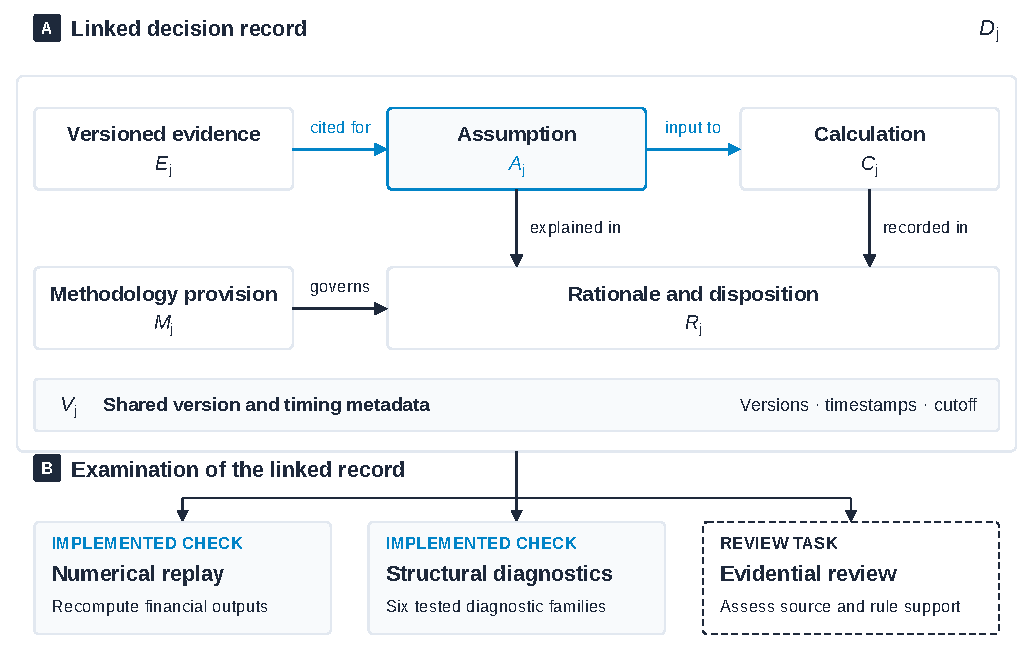
\includegraphics[width=175mm]{figures/Figure_1_Record_and_Review.pdf}}
  \caption{Decision record and review controls. Evidence, assumptions, calculations, methodology provisions, rationale and disposition, and version/timing metadata form a linked decision record. Numerical replay and structural diagnostics are implemented checks. Evidential review examines source support and governing treatment. Arrows in panel A label conceptual relationships. Source: author's own work.}
  \label{fig:architecture}
\end{figure}
\FloatBarrier

\subsection{Information timing and admissibility}

Each case has an information cutoff $t_c$ and an assessment or payment date $t_d$ . A document can support the decision only if it belongs to the information set available by $t_c$ . A future payment can be modeled when its contractual basis is documented by $t_c$ , but an event observed only after $t_c$ belongs to a later case version. This prevents hindsight from determining an earlier analytical judgment. The methodology status variable $m_j$ takes one of three values: 0 for ordinary application, 1 for judgment within an explicitly authorized range, and 2 for a departure requiring additional justification or escalation. The status is derived from the supplied methodology rule, not from whether the resulting credit outcome is favorable or adverse.

\subsection{Synthetic credit-risk families}

Three families each contain favorable, unchanged and adverse branches, giving nine financial configurations. Monetary amounts and outputs below are in SAR millions. The exposure family varies exposure at default while fixing probability of default (PD), loss given default (LGD) and discounting. Its one-period expected loss is

\begin{equation}\label{eq:one-period}\mathrm{EL}=\mathrm{EAD}\times\mathrm{PD}\times\mathrm{LGD}.\end{equation}

Here, $\mathrm{EAD}$ is exposure at default, $\mathrm{PD}=0.02$ is the conditional default probability and $\mathrm{LGD}=0.40$ is the loss fraction. With unit discounting, exposures of 60, 100 and 140 produce expected losses of 0.48, 0.80 and 1.12 in the favorable, unchanged and adverse branches; baseline loss is 0.80.

Refinancing changes the duration of the original lender's exposure. Default occurs within each period; conditional termination follows at its end. Expected loss therefore accumulates only while exposure survives both prior default and termination. For two periods with constant exposure, unit discounting and conditional default probability $p$, the baseline is

\begin{equation}\label{eq:two-period}\mathrm{EL}=\mathrm{EAD}\times\mathrm{LGD}\left[p+(1-p)p\right].\end{equation}

With $\mathrm{EAD}=100$, $\mathrm{LGD}=0.40$ and $p=0.02$, baseline and unchanged loss equal 1.584. Favorable refinancing terminates exposure after period one, giving 0.80. The adverse branch retains exposure through period three, giving $100(0.40)[0.02+0.98(0.02)+0.98^2(0.02)]=2.35232$. The three-period exposure vectors are $(100,0,0)$, $(100,100,0)$ and $(100,100,100)$, with termination vectors $(1,0,0)$, $(0,1,0)$ and $(0,0,1)$ for favorable, unchanged and adverse branches respectively.

Sponsor-support calculations use operating cash 85, eligible reserve 5 and debt service 100 on day~0. The baseline and unchanged branch admit eligible support of 10 arriving on day~$-5$, giving resources of 100 and headroom of 0. The favorable branch admits 20 on day~$-5$, giving resources of 110 and headroom of 10. The adverse branch schedules 20 on day~$+5$, leaving resources of 90 and headroom of $-10$ at payment. Figure~\ref{fig:support} isolates the fixed-20 timing comparison; the unchanged branch uses 10.

\begin{figure}[H]
  \centering
  \makebox[\linewidth][c]{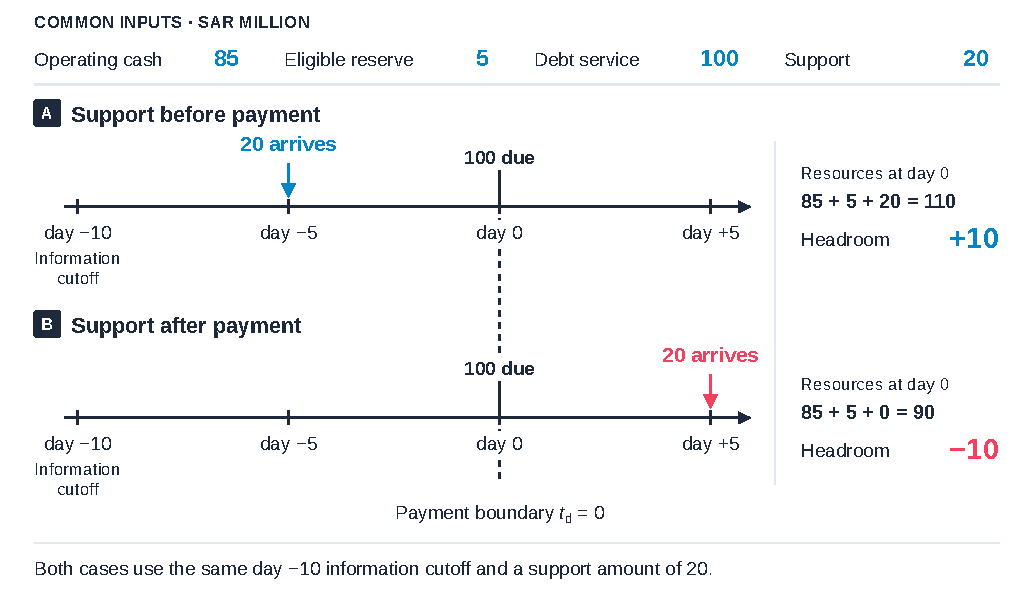
\includegraphics[width=175mm]{figures/Figure_2_Support_Timing.pdf}}
  \caption{Sponsor-support timing. The same support amount of 20 arrives on day~$-5$ or day~$+5$ relative to payment on day~0. Resources at payment are 110 or 90, giving headroom of $+10$ or $-10$. Operating cash is 85, eligible reserves are 5 and debt service is 100. All amounts are SAR million; both cases use the day~$-10$ information cutoff. Source: author's own work.}
  \label{fig:support}
\end{figure}
\FloatBarrier

\Needspace{10\baselineskip}
\subsection{Case bank and fault classes}

The case bank crosses three credit families, three financial effects, three methodology statuses (ordinary application, permitted judgment and departure) and two evidence states (sufficient and unresolved). Its $3\times3\times3\times2=54$ design cells contain 18 cells per family. Each cell produces a supporting-attribution control (suffix -C) and a semantic-attribution defect (suffix -X), giving 108 stored variants. Six single-rule mutations of each control generate $54\times6=324$ structural perturbations. All 54 controls are included. The supplementary \nolinkurl{data/case_design_grid.csv} specifies every cell.

Structural faults violate identifier, link, cycle, cutoff, digest or metadata constraints. Semantic defects redirect an assertion to a structurally valid source that fails to support it. Both records retain the same financial inputs and calculations. The pair below makes this distinction inspectable.

\subsubsection{An instantiated source-to-disposition chain}\label{sec:worked-record}

The archived D037-C/D037-X pair concerns the favorable sponsor-support branch with resolved confirmation and ordinary methodology application. At the day~$-10$ information cutoff, candidate source E0 version~1.0 is already available from day~$-11$. Its passage records \texttt{``support\_amount'': ``20''} and \texttt{``arrival\_day'': -5}, followed by ``The required confirmation is resolved.'' The assumption is to include this documented support in resources for the day~0 payment.

The constructed provision M1:1.0 states: ``M1 authorizes an ordinary documentary update of support availability at the debt-payment cutoff when its conditions are established.'' Calculation C1 applies the baseline E1 and candidate E0 inputs: $85+5+10-100=0$ baseline headroom and $85+5+20-100=10$ candidate headroom. Review record R1 records review under M1. In D037-C, rationale A1 cites E0 for the inputs and condition, M1 and R1 for authority, and C1 for the financial consequence. Disposition J1 states: ``Accept the candidate treatment under the supplied rule.''

D037-X redirects A1 and its evidence link to E2 version~0.9, the older onboarding schedule. E2 states: ``No subsequent utilization instruction, settlement confirmation or support amendment is recorded in this schedule.'' The pair retains identical source passages, rule, calculation and disposition; both linked sources exist and precede the cutoff. The changed attribution is unsupported because E2 lacks the candidate support amendment. These aliases are specific to D037; source labels are shuffled across design cells. Figure~\ref{fig:d037-attribution} displays the source-attribution comparison.

\begin{figure}[H]
  \centering
  \makebox[\linewidth][c]{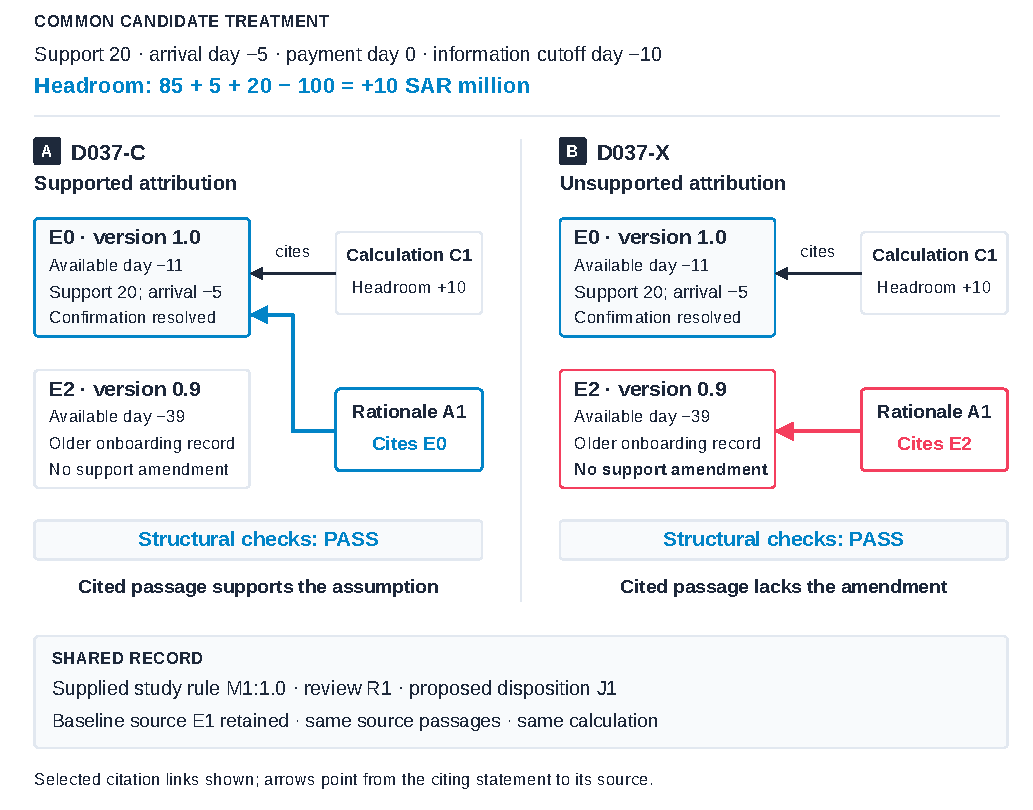
\includegraphics[width=175mm]{figures/Figure_3_D037_Source_Attribution.pdf}}
  \caption{D037 source-attribution comparison. Both records retain the candidate calculation link C1 $\rightarrow$ E0. The rationale cites E0 in D037-C and E2 in D037-X. E0 records the candidate support and confirmation; E2 lacks the amendment. Both pass structural validation. Source-support annotations describe the cited passages. The full record also retains the baseline calculation link C1 $\rightarrow$ E1. Source: author's own work.}
  \label{fig:d037-attribution}
\end{figure}
\FloatBarrier

\section{Computational methodology and reproducibility}

\subsection{Structural validation rules}

The validator first requires the top-level keys \nolinkurl{case_id}, \nolinkurl{cutoff}, \nolinkurl{statements}, \nolinkurl{asserted_links}, \nolinkurl{provenance} and \nolinkurl{decision_metadata}; a missing key returns a \nolinkurl{missing:} diagnostic immediately. Canonical records supply statement identifiers and text. Six families govern the tested structural perturbations:
\begin{enumerate}[leftmargin=*,nosep]
\item Identifier uniqueness compares all statement \nolinkurl{id} values and flags duplicates.
\item Reference resolution checks that both endpoints of each \nolinkurl{asserted_links} pair occur among statement identifiers; self-links also produce a diagnostic.
\item Acyclicity checks the directed asserted-link graph over existing identifiers for dependency cycles.
\item Timing checks every evidence statement: \nolinkurl{available_day} must be no later than \nolinkurl{cutoff} and no earlier than \nolinkurl{issued_day}. The stored \nolinkurl{effective_day} is not compared with the cutoff.
\item Source integrity compares the SHA-256 digest of UTF-8-encoded \nolinkurl{text} with the stored \nolinkurl{sha256} value.
\item {\raggedright Decision-metadata presence checks membership of eleven keys: \texttt{methodology}, \texttt{provision}, \texttt{affected\_assumption}, \texttt{calculation\_ref}, \texttt{rationale\_ref}, \texttt{owner}, \texttt{timestamp\_day}, \texttt{challenge}, \texttt{disposition\_ref}, \texttt{approval\_ref} and \texttt{review\_trigger}.\par}
\end{enumerate}

Before checking evidence dates and digests, the function requires \nolinkurl{version}, \nolinkurl{issuer}, \nolinkurl{passage}, \nolinkurl{entity}, \nolinkurl{sha256}, \nolinkurl{issued_day}, \nolinkurl{effective_day} and \nolinkurl{available_day}. A missing key flags an incomplete source and skips that source's date and digest checks. Graph reference resolution applies to asserted-link endpoints; metadata checks establish key presence rather than populated values or resolution of metadata reference targets.

For the six tested families, let $g_r(x)\in\{0,1\}$ indicate failure of family $r$ in record $x$. Their combined alert is

\begin{equation}\label{eq:validator}G(x)=\mathbb{I}\!\left(\sum_{r=1}^{6}g_r(x)>0\right).\end{equation}

Here, $\mathbb{I}(\cdot)$ is the indicator function. Clean controls satisfy $G(x)=0$. The admission, incomplete-source and additional date/self-link diagnostics above specify the surrounding implementation contract; the reported mutation corpus targets the six families.

\subsection{Deterministic financial recomputation}

Each stored variant contains baseline and candidate financial values generated from explicit inputs. The audit recomputes those outputs independently from the stored results and defines numerical discrepancy

\begin{equation}\label{eq:discrepancy}\Delta_i=\left|\widehat{y}_i-y_i\right|.\end{equation}

where $y_i$ is the stored output and $\widehat{y}_i$ is the recomputed output. A financial check passes when $\Delta_i$ $\leq$ $10^{-9}$ in the internal numerical units. Recomputation covers all nine branches in Section~3.3, including one-, two- and three-period refinancing and the distinct 10-million support baseline.

\subsection{Controlled structural perturbations}

For each of the 54 supporting-attribution -C controls defined in Section 3, the audit creates six independent in-memory perturbations, one for each diagnostic family. The underlying stored files are not modified. The resulting structural test corpus therefore contains $54\times 6$ = 324 perturbed records. Each perturbation changes only the targeted structural condition. This design tests whether the intended rule fires without requiring a probabilistic sampling interpretation. Component ablation suppresses the diagnostic output of one family at a time while leaving the record, other rules and test corpus unchanged. If $G_{-r}(x)$ is the validator with diagnostic family $r$ suppressed, the finite-corpus coverage is

\begin{equation}\label{eq:ablation}\mathrm{Cov}_{-r}=\frac{1}{324}\sum_{i=1}^{324}G_{-r}(x_i).\end{equation}

The full validator coverage is defined analogously using $G$. Because the corpus is exhaustive for the constructed single-fault perturbations, these quantities are exact corpus proportions rather than estimates of a population sensitivity.

\subsection{Comparator and semantic controls}

The decision-metadata key-presence configuration runs the full validator and retains only \nolinkurl{incomplete_decision_metadata} diagnostics. For admitted records, its alert tests whether any of the eleven nested keys in Section~4.1 is missing. Removing \nolinkurl{owner} therefore triggers this configuration; removing top-level \nolinkurl{cutoff} produces a \nolinkurl{missing:cutoff} diagnostic that its filter discards. The comparison measures diagnostic filtering within the same implementation.

The 54 semantic-defect records preserve the checked structural predicates while redirecting an attribution to a non-supporting source, as illustrated by D037-X. Their expected structural outcome is no alert. They isolate evidential support from graph and metadata conformance.

\subsection{Reproducibility environment}

The release includes the synthetic case definitions, source manifest, deterministic calculation code, validator, perturbation generator, ablation analysis and output tables. The computational audit reads fixed inputs, verifies file digests, performs recomputation, executes perturbations and exports machine-readable results. The analysis does not require proprietary rating-agency systems or confidential committee records. Random sampling is not used in the reported structural coverage results.

The research archive was independently executed in a separate working copy on 14 November 2026. Verification used the archived test suite, deterministic audit and output-checking scripts, with regenerated artifacts compared against the original released outputs. The protocol records unit-test outcomes, financial recomputation, structural diagnostic counts, ablations and matching output files. The audit executes the supplied implementation; it does not introduce a second implementation of the credit-risk calculations.

\section{Results}

\subsection{Case-bank integrity and financial recomputation}

The executed audit covered all 108 stored synthetic case variants. Across the case bank, 216 stored baseline and candidate financial outputs were recomputed independently. Every recomputed value matched the stored value within the $10^{-9}$ tolerance, producing zero numerical discrepancies. These results cover the exposure-change, refinancing-termination and sponsor-support timing cases specified in Section 3.

\par\noindent\textit{[Insert Table II about here.]}\refstepcounter{table}\label{tab:computational-audit}\par

Refinancing reduces expected loss from 1.584 to 0.80 under one-period termination and increases it to 2.35232 under three-period retention. The changes, $-0.784$ and $+0.76832$ SAR million, differ because the additional period is survival weighted. For support, the fixed-20 timing contrast yields headroom of $+10$ or $-10$; the unchanged 10-million branch yields zero. All nine configurations are specified in Section~3.3.

\subsection{Structural fault detection}

The full validator alerted on all 324 injected structural perturbations and produced no alerts on the 54 unmodified controls (Table~\ref{tab:computational-audit}). Each controlled perturbation activated its intended diagnostic family. The decision-metadata key-presence configuration alerted on the 54 missing-owner perturbations and on none of the other 270 structural perturbations.

\subsection{Diagnostic-family ablation}

Suppressing any one of the six diagnostic families reduced structural alert coverage from 100\% to 83.33\%, an absolute reduction of 16.67 percentage points. All 54 newly missed perturbations belonged to the suppressed diagnostic's own fault family; coverage of the other five families remained complete. Figure~\ref{fig:ablation} displays this one-to-one pattern.

\begin{figure}[H]
  \centering
  \makebox[\linewidth][c]{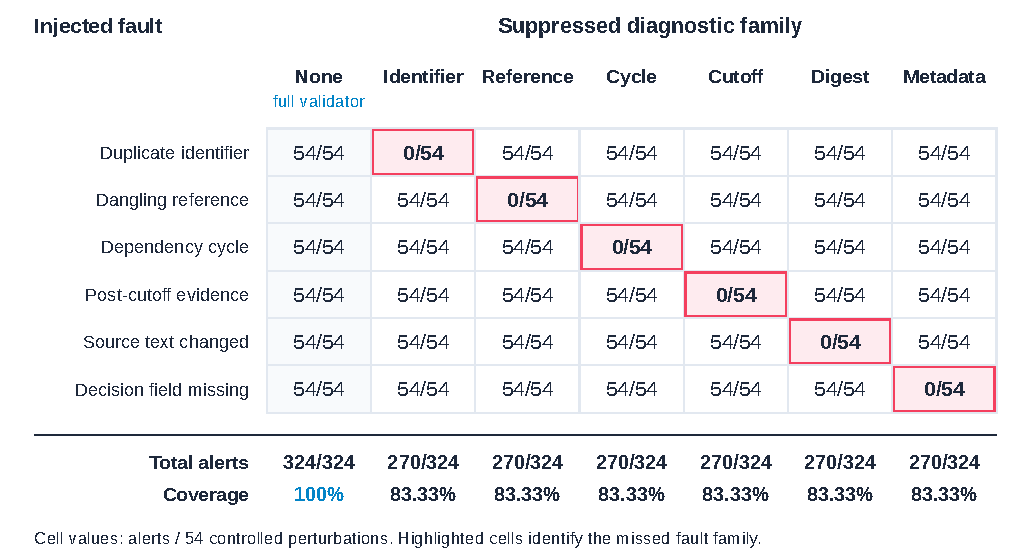
\includegraphics[width=175mm]{figures/Figure_4_Diagnostic_Ablation.pdf}}
  \caption{Diagnostic-family ablation matrix. Rows identify injected structural faults; columns identify the diagnostic output suppressed. Each matrix cell reports alerts among 54 perturbations. The full validator detects 324/324 faults. Suppressing one diagnostic family leaves its 54 faults undetected, giving 270/324 coverage (83.33\%). Counts are exact over the fixed corpus. Source: author's own work.}
  \label{fig:ablation}
\end{figure}
\FloatBarrier

\subsection{Semantic attribution boundary}

All 54 deliberately misleading source-attribution records passed structural validation, as designed. Their identifiers were unique, asserted-link endpoints resolved, digests matched, evidence dates met the checks and required metadata keys existed. In the D037 pair (Section~\ref{sec:worked-record}), changing the attribution from E0 to E2 preserves all those conditions while removing support for the candidate assumption. Figure~\ref{fig:architecture} separates that evidential assessment from structural checking.

\subsection{Independent computational reproduction}

The separately executed 14 November 2026 verification passed all 12 archived unit tests. The reproduced audit matched the 216 financial outputs, 324 structural-fault alerts and absence of alerts on the 54 clean controls. As designed, none of the 54 semantic-attribution records triggered a structural alert. All eight regenerated computational output files were byte-for-byte identical to the corresponding archived files. These checks verify repeatability of the released deterministic analysis in the separate execution.

\section{Discussion}

\subsection{What the evaluated controls establish}

Financial replay, fault detection and ablation make each implemented control inspectable on the fixed corpus. The input condition, violated constraint and resulting alert identify a defined failure class; suppressing its diagnostic exposes the corresponding 54 faults.

The 54 misleading attributions preserve the checked identifiers, asserted links, digests, dates and metadata keys. The D037 pair locates the error in the rationale's source selection, making evidential support a separately inspectable decision.

\subsection{Operational interpretation for methodology review}

Identifier and asserted-link endpoint checks detect duplicate labels and missing graph targets; cycle checks detect circular dependencies. Evidence-date checks compare availability with issue and cutoff dates, and digest checks detect source-text changes. The metadata diagnostic detects absent keys, including a missing owner, rather than assessing their values or referenced targets. Financial replay verifies the numerical consequence. Each output therefore identifies the specific predicate tested in Section~4.1.

This control-purpose mapping provides a bounded technical response to the operational agenda identified by \citet{castro2026}. A prospective workflow could run the structural checks before a decision enters review and rerun them when an evidence or methodology version changes. Subsequent review could replay the calculation and inspect the recorded rationale and disposition. The temporal placement of those checks is an implementation proposal grounded in their evaluated functions.

Prorokowski's operational observations make the distinction between source identification and substantive relevance particularly pertinent \citep{prorokowski2026}. The rating application introduces its own review objects: the financial assumption, the governing methodology and the analyst's disposition. The semantic controls turn the difference between a present justification and a supported justification into an explicit test condition. This complements the disclosure-quality finding of \citet{roncato2026} by specifying a decision-level failure mode that can remain hidden behind complete documentation.

\subsection{Relationship to existing credit-governance frameworks}

The contribution follows the task-oriented logic established by \citet{bucker2022} and \citet{xie2026}: evaluation must match the purpose for which an analytical artefact is used. It sits within the governed-decision perspective of \citet{khalili2026} and the prior financial-decision provenance implementation of \citet{huynh2021}. It is also compatible with graph-based constraint checking using the established SHACL standard \citep{shacl2017}. Here, the specific artefact is the recorded application of a credit-rating methodology; the evaluated properties are financial reconstructability and six structural diagnostic behaviours. The 54 semantic-attribution records identify the exact boundary between an internally consistent record and a supported analytical judgment. This is the relevant boundary for the independently adjudicated source-to-methodology question: a reviewer needs to check the passage, the cutoff date, the applicable methodology version and the financial treatment together. The existing experiment supplies a reproducible test object and a task-specific control-characterisation result at that boundary.

The record links an exposure change to its source and recomputed loss, distinguishes anticipated refinancing from the event terminating exposure, and connects sponsor-support conditions and timing to payment-date liquidity. Each relationship lets a reviewer trace a judgment back to its evidence and forward to its numerical consequence.

\section{Conclusion}

The study establishes a reproducible decision-level control specification for examining credit-rating methodology applications. Versioned records connect dated source evidence to assumptions, financial consequences, governing provisions and analytical dispositions. The fixed-corpus tests reproduce 216 financial values, detect all 324 injected single-fault structural violations and generate no alerts on 54 unmodified controls. Fifty-four misleading source-attribution records remain structurally valid, showing precisely where documentary support must be assessed as a distinct review decision.

This measured separation of numerical replay, structural conformance and evidence-to-methodology assessment makes the paper's operational-compliance contribution specific and verifiable. It identifies which record properties the implemented controls establish and supplies the reproducible record and failure conditions on which substantive methodological judgment can be examined.

\section*{Data and code availability}

The computational reproducibility supplement contains the 108 synthetic records, design grid, calculation and validation scripts, and machine-readable outputs. The separate verification bundle contains the independent report and execution logs dated 14 November 2026. Original inputs, code and verification records are unchanged.

\section{Limitations}

The case bank is synthetic; its validator and semantic attribution defects were developed within the same research programme. The equal allocation of 54 isolated faults to each diagnostic family explains the uniform 16.67-percentage-point reduction under ablation, rather than estimating fault prevalence or operational importance. The decision-metadata comparator filters the full validator's diagnostics; performance against independently implemented graph-validation or provenance systems remains unmeasured. The computational reproduction reruns archived scripts and verifies their outputs; it is not an independent implementation of the rules.

The evaluated outputs characterize numerical and structural record properties. They do not measure comparative reviewer accuracy for source-to-methodology judgments under matched narrative, flat-register and linked-record presentations, or rating accuracy, committee consistency, review duration and organisational effectiveness. Interacting methodology-version, timing and source-support faults have not been evaluated. Operational deployment requires institution-specific methodology mappings, access controls and confidentiality arrangements.

The focused literature synthesis connects JFRC and related credit-governance research. Transferring findings from banking compliance, sustainability reporting, cryptocurrency regulation and corporate disclosure to rating-methodology review is an analytical synthesis. Central JFRC claims were checked in full text; some complementary studies were assessed through abstracts and selected sections. The FCA observations concern UK supervisory samples. Generalisation requires independent cases and evaluation in the intended setting.

\begingroup
\setstretch{1.0}
\setlength{\bibsep}{5pt}
\interlinepenalty=10000
\bibliographystyle{jfrc_harvard_doi}
\bibliography{references}
\endgroup
\end{document}
